%% LyX 2.2.3 created this file.  For more info, see http://www.lyx.org/.
%% Do not edit unless you really know what you are doing.
\documentclass[twoside,american]{report}
\usepackage[sc]{mathpazo}
\usepackage[scaled=0.9]{helvet}
\renewcommand{\ttdefault}{lmtt}
\usepackage[T1]{fontenc}
\usepackage[latin9]{inputenc}
\usepackage[a4paper]{geometry}
\geometry{verbose,lmargin=1.7cm,rmargin=1.7cm}
\usepackage{fancyhdr}
\pagestyle{fancy}
\setcounter{secnumdepth}{0}
\setcounter{tocdepth}{3}
\setlength{\parskip}{\smallskipamount}
\setlength{\parindent}{0pt}
\usepackage{babel}
\usepackage{float}
\usepackage{enumitem}
\usepackage{graphicx}
\usepackage[unicode=true,
 bookmarks=true,bookmarksnumbered=false,bookmarksopen=false,
 breaklinks=false,pdfborder={0 0 1},backref=false,colorlinks=false]
 {hyperref}

\makeatletter
%%%%%%%%%%%%%%%%%%%%%%%%%%%%%% Textclass specific LaTeX commands.
\newlength{\lyxlabelwidth}      % auxiliary length 

%%%%%%%%%%%%%%%%%%%%%%%%%%%%%% User specified LaTeX commands.
% Customization file for the titlepage and document
%************************************************************
% Required stuff
%************************************************************
\usepackage{graphicx}
\usepackage{euler}
\usepackage[detect-all]{siunitx}
\usepackage{sectsty}
\usepackage[font={footnotesize }]{caption}
\usepackage{multicol}
\usepackage{prettyref}

\allsectionsfont{\rmfamily}

% Page customization
\usepackage{fancyhdr}
\pagestyle{fancy}

% Color
\usepackage{color}
\definecolor{light-gray}{gray}{0.85}
\definecolor{dark-gray}{gray}{0.75}

\fancyhead{}  % clear all header fields
\fancyhead[LO,RE]{\rule[-2ex]{0pt}{2ex}\fontsize{9}{11} \selectfont \myPhase : \myTitle}
\fancyhead[CO,CE]{\fontsize{9}{11} \selectfont \myIPT}
\fancyfoot{}  % clear all footer fields
\fancyfoot[LO,LE]{\fontsize{8}{11} \selectfont {\sscap{Website}} : \url{https://github.com/fcuzzocrea/MSAS2017}}
\fancyfoot[RO,LE]{\fontsize{5}{11} \selectfont 
\includegraphics[height=0.18cm]{gfx/CC}  This work is licensed under a Creative Commons Attribution-ShareAlike 4.0 International License.}
\fancyheadoffset[LE,RO]{0.2pt}
\renewcommand{\headrulewidth}{0.2pt}
\renewcommand{\footrulewidth}{0.2pt}
\renewcommand{\headrule}{\hbox to\headwidth{%
   \leaders\hrule height \headrulewidth\hfill}}
\renewcommand{\footrule}{\hbox to\headwidth{%
    \leaders\hrule height \headrulewidth\hfill}}
\hypersetup{colorlinks=true, linkcolor=blue ,linktoc=page,citecolor=black}

%************************************************************
% Redefining numbering for sections
%************************************************************
%\renewcommand*\thesection{\arabic{section}}

%************************************************************
% Cross reference set-up
%************************************************************
\newrefformat{tab}{Table\,\ref{#1}}
\newrefformat{fig}{Figure\,\ref{#1}}
\newrefformat{eq}{Eq.\,\textup{(\ref{#1})}}
\newrefformat{sec}{Sec.\,\ref{#1}}
\newrefformat{sub}{Sec.\,\ref{#1}}

%************************************************************
% Fancy stuff
%************************************************************
\newcommand{\titlecap}[1]{\Huge{\textrm{#1}}}
\newcommand{\subtitlecap}[1]{\Large{\textsc{#1}}}
\newcommand{\sscap}[1]{\textbf{#1}}
\newcommand{\strong}[1]{\textbf{#1}}
\setlength{\headheight}{60pt} %%or

%************************************************************
% Helpful stuff to modify here, not in the LyX Document
%************************************************************
\newcommand{\myDate}{\today}
\newcommand{\myGroup}{}
\newcommand{\myUrl}{\url{https://github.com/fcuzzocrea/MSAS2017}}
\newcommand{\myUni}{}

\newcommand{\myPhase}{Modeling and Simulation of Aerospace Systems}
\newcommand{\myProject}{}
\newcommand{\myIPT}{}
\newcommand{\myTitle}{LISA Pathfinder Final Report}
\newcommand{\myAuthorf}{Alfonso Collogrosso}
\newcommand{\myAuthors}{Francescodario Cuzzocrea}
\newcommand{\myAuthort}{Andrea Mastrantuono}
\newcommand{\myEmail}{}

\newcommand{\mail}[1]{\href{mailto:#1}{\texttt{#1}}}

\setlength{\textfloatsep}{\baselineskip}

\makeatother

\begin{document}
\thispagestyle{empty}
\pdfbookmark{Titlepage}{Titlepage}

\vspace{3cm}
\begin{center}
\bigskip
\Large{\myDate}
\vspace{0.5cm}

{\titlecap{\myProject} \\
\vspace{0.3cm}
\titlecap{\myPhase}}\\
\vspace{0.4cm}
\rule{\linewidth}{0.5mm}
\titlecap{\myTitle}


\vfill

\begin{tabular}{cc}
\hspace{2.5cm}
\parbox{0.3\textwidth}{
\includegraphics[height=7cm]{gfx/Polimi}}
&
\parbox{0.7\textwidth}{{\subtitlecap{\myIPT}} \\

					{\normalsize
						\textrm{\myGroup \\
						\myUni \\
						\textbf{Author}: {\myAuthorf}\\
						\textbf{Author}: {\myAuthors}\\
						\textbf{Author}: {\myAuthort}}}}\\
\end{tabular}
\end{center}
\clearpage


%*******************************************************
% Titleback
%*******************************************************
\thispagestyle{empty}

\hfill
\vspace{5cm}
\strong{ }\\
The LISA scientific space mission will detect gravitational waves by measuring the relative displacement of a pairs of free floating test masses set into geodesic motion on-board of three spacecraft. Inside each satellite, the injection of the test masses from the caged configuration into the geodesic trajectory will be performed by the Grabbing Positioning and Relased Mechanism (GPRM). To provide a successful injection, the test masses must be relased with a minimal residual velocity against the adhesion with the holding device.
In the following document we will proceed trough the derivation and the integration of the system of linear ODEs that describes the forementioned grabbing positioning and relase mechanism.

\vfill

\begin{multicols}{2}
\medskip
\noindent{\sscap{Website}}: \\
\url{https://github.com/fcuzzocrea/MSAS2017}


\medskip
\noindent{\sscap{}} \\
\mail{\myEmail}
\vfill
\columnbreak

\end{multicols}
\vspace{1cm}
\hrule
\bigskip
\clearpage


\pagenumbering{roman}

\tableofcontents{}

\clearpage{}

\pagenumbering{arabic}

\setcounter{page}{1}

\chapter{Modeling}

\newpage{}

\section{The real system}

The LISA Pathfinder grabbing position and relase mechanism (abbreviated
as GPRM) is the system aimed to lock and relase the test mass (from
now on TM) into the spacecraft. 

In fact, forementioned TM has to be relased with a nearly zero velocity
with respect to the transport spacecraft to be correctly injected
into a geodesic trajectory (wich is what we aim for). 

This task can be relatively complex, if we think of the possible interactions
that develope with the support, and because of the electrostatic aspects
that may generate disturbing forces. Also, least but not last, the
quality of the surface of the test mass and of the grabbing finger
should be take into account. The GPRM mechanism is sketched in Fig
1.

\begin{figure}[H]
\begin{centering}
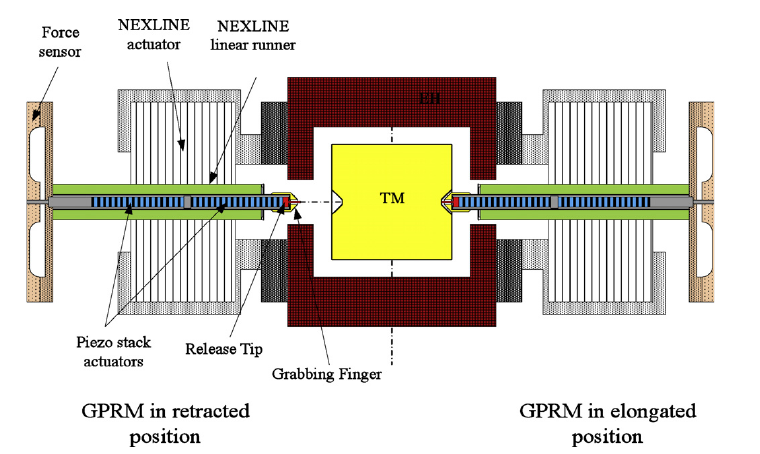
\includegraphics[scale=0.7]{gfx/GPRM}
\par\end{centering}
\caption{GPRM Mechanism}

\end{figure}

It's main parts are :
\begin{itemize}
\item \textit{Grabbing Finger} : holds the TM and positions it prior relase;
\item \textit{Finger Tip} : last contact part that pons the TM in position
before fast retraction for relase;
\item \textit{Low Voltage Piezo Actuator} : used for the positioning and
fast Finger Tip relase;
\item \textit{NEXLINE actuator} : used for Grabbing Finger movement;
\item \textit{Displacemente Sensor} : to measure the axial force acting
between the mechanism contacting interface;
\end{itemize}

\subsection{Main Task}

The model of the injection procedure consist of three parts. The GPRM
(sketched in Fig. 1), the adhesion phenomenon and the TM motion equations.
Two opposite GPRMs are operated simultaneously in order to hold the
TM with the Grabbing Fingers in the center of the Electriode Housing
(EH). From this configuration, the procedure can be cosidered symmetrical,
as the two mechanism are commanded in the same way :
\begin{itemize}
\item \textbf{Pre-launch and launch phase}
\begin{enumerate}
\item The TM is held by the Caging Mechanism (CM) at the eight corners;
\end{enumerate}
\item \textbf{TM Relase from CM}
\begin{enumerate}
\item The Grabbing Finger is in contract with the TM and the tip is fully
retracted;
\end{enumerate}
\end{itemize}
The contact between the GF and the TM has to perform the following
functions :
\begin{description}
\item [{-}] Fix the TM during the relase of the CM;
\item [{-}] Centre the TM in the EH;
\item [{-}] Orient the TM with respect to the EH;
\end{description}
This contact however not suitable for an undisturbate relase for geodesic
injection. The relase tip must thus take over the TM pinning before
relase. 
\begin{itemize}
\item \textbf{Pass Over}
\begin{enumerate}
\item The RT moves forward until a contact force is recorded \textbackslash{}item
The GF is retracted a small amount to compensate for the movemente
of the RT;
\item The force is then reduced to the lowes acceptable level that still
controls the postion of the TM;
\item TM relase is performed by means of a fast contraction of the linear
piezo actuator, wich also commands the retraction of the tips;
\item The TM is capture by the drag-free attitude and control system and
take finally to the nominal center of its housing;
\end{enumerate}
\end{itemize}
We must pay attention to the fact that in presence od adhesion the
fast retraction may cause a momentum transfer from the RTs to TM. 

\subsection{The Physical System}

\subsection{The Mathematical Model}
\end{document}
